\documentclass[10pt,a4paper]{article}

\usepackage[utf8]{inputenc}
\usepackage[T1]{fontenc}
\usepackage[margin=1.5cm]{geometry}
\usepackage{amsmath,amssymb}
\usepackage{tikz}
\usetikzlibrary{positioning,calc,arrows.meta,shapes.geometric,matrix,fit,decorations.pathreplacing}
\usepackage{xcolor}
\usepackage{colortbl}
\usepackage{listings}
\usepackage{tcolorbox}
\tcbuselibrary{breakable}
\usepackage{hyperref}
\usepackage{multicol}
\usepackage{graphicx}

\lstset{
    language=C,
    basicstyle=\ttfamily\scriptsize,
    backgroundcolor=\color{gray!10},
    keywordstyle=\color{blue},
    commentstyle=\color{gray},
    stringstyle=\color{red},
    numbers=left,
    numberstyle=\tiny,
    breaklines=true,
    frame=single,
    tabsize=4,
    showstringspaces=false,
    inputencoding=utf8,
    extendedchars=true,
    literate={é}{{\'e}}1 {è}{{\`e}}1 {à}{{\`a}}1 {ç}{{\c{c}}}1 
             {ê}{{\^e}}1 {î}{{\^i}}1 {ô}{{\^o}}1 {û}{{\^u}}1 {ù}{{\`u}}1
             {É}{{\'E}}1 {È}{{\`E}}1 {À}{{\`A}}1 {Ç}{{\c{C}}}1
             {Ê}{{\^E}}1 {Î}{{\^I}}1 {Ô}{{\^O}}1 {Û}{{\^U}}1 {Ù}{{\`U}}1
             {ë}{{\"e}}1 {ï}{{\"\i}}1 {ö}{{\"o}}1 {ü}{{\"u}}1
             {Ë}{{\"E}}1 {Ï}{{\"I}}1 {Ö}{{\"O}}1 {Ü}{{\"U}}1
             {œ}{{\oe}}1 {Œ}{{\OE}}1 {æ}{{\ae}}1 {Æ}{{\AE}}1
}

\newtcolorbox{definitionbox}[1]{colback=blue!5,colframe=blue!75!black,fonttitle=\bfseries,title=#1,breakable}
\newtcolorbox{examplebox}[1]{colback=green!5,colframe=green!50!black,fonttitle=\bfseries,title=#1,breakable}
\newtcolorbox{warningbox}[1]{colback=red!5,colframe=red!75!black,fonttitle=\bfseries,title=#1,breakable}
\newtcolorbox{techbox}[1]{colback=orange!5,colframe=orange!75!black,fonttitle=\bfseries,title=#1,breakable}
\newtcolorbox{infobox}[1]{colback=cyan!5,colframe=cyan!75!black,fonttitle=\bfseries,title=#1,breakable}

\title{\textbf{Chapitre 1 : Représentation Numérique}\\
\large Binaire, Hexadécimal, Entiers et Flottants}
\author{Dr. El Hadji Bassirou TOURÉ\\
Département de Mathématiques et Informatique\\
Faculté des Sciences et Techniques\\
Université Cheikh Anta Diop de Dakar}
\date{}

\begin{document}
\maketitle

\section{Systèmes de Numération}

\subsection{Base Binaire}

\begin{definitionbox}{Notation binaire}
En base 2, chaque position représente une puissance de 2. Un nombre binaire $b_{n-1}b_{n-2}...b_1b_0$ correspond à $\sum_{i=0}^{n-1} b_i \cdot 2^i$ où $b_i \in \{0,1\}$. Le bit de poids fort (MSB) est à gauche, le bit de poids faible (LSB) à droite.
\end{definitionbox}

\begin{center}
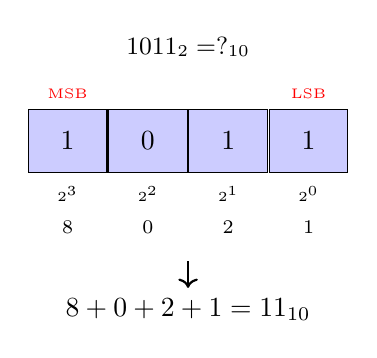
\begin{tikzpicture}[scale=0.85]
\node at (1.8,2.2) [font=\small] {$1011_2 = ?_{10}$};
\foreach \i/\bit/\val in {3/1/8, 2/0/0, 1/1/2, 0/1/1} {
    \node[rectangle,draw,fill=blue!20,minimum width=1cm,minimum height=0.8cm] at ({(3-\i)*1.2},0.8) {\bit};
    \node at ({(3-\i)*1.2},0) [font=\tiny] {$2^{\i}$};
    \node at ({(3-\i)*1.2},-0.5) [font=\scriptsize] {\val};
}
\node at (0,1.5) [font=\tiny,red] {MSB};
\node at (3.6,1.5) [font=\tiny,red] {LSB};
\draw[->,thick] (1.8,-1) -- (1.8,-1.4) node[below] {$8+0+2+1=11_{10}$};
\end{tikzpicture}
\end{center}

\begin{techbox}{Conversion décimal $\rightarrow$ binaire}
Division successive par 2, en conservant les restes. Lire les restes de bas en haut (dernier reste = MSB).
\end{techbox}

\begin{center}
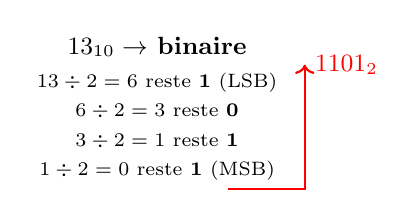
\begin{tikzpicture}[scale=0.75]
\node at (0,2.8) [font=\small\bfseries] {$13_{10} \rightarrow$ binaire};
\node at (0,2.2) [font=\scriptsize] {$13 \div 2 = 6$ reste $\mathbf{1}$ (LSB)};
\node at (0,1.7) [font=\scriptsize] {$6 \div 2 = 3$ reste $\mathbf{0}$};
\node at (0,1.2) [font=\scriptsize] {$3 \div 2 = 1$ reste $\mathbf{1}$};
\node at (0,0.7) [font=\scriptsize] {$1 \div 2 = 0$ reste $\mathbf{1}$ (MSB)};
\draw[->,thick,red] (1.2,0.4) -- (2.5,0.4) -- (2.5,2.5) node[right,font=\small] {$1101_2$};
\end{tikzpicture}
\end{center}

\subsection{Base Hexadécimale}

\begin{definitionbox}{Notation hexadécimale}
Base 16 utilise les symboles 0-9 et A-F (A=10, B=11, C=12, D=13, E=14, F=15). Préfixe \texttt{0x} en C. Chaque chiffre hex = 4 bits exactement.
\end{definitionbox}

\begin{center}
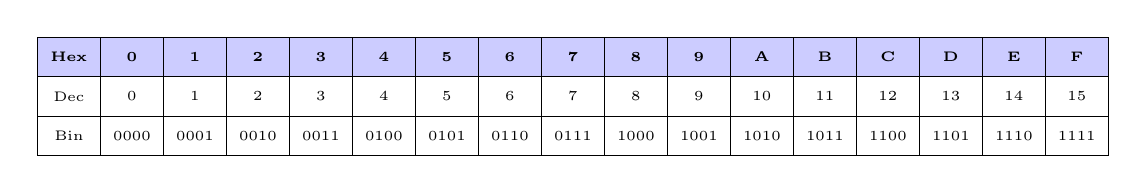
\begin{tikzpicture}[scale=0.7]
\matrix (m) [matrix of nodes,
    nodes={rectangle,draw,minimum width=0.8cm,minimum height=0.5cm,anchor=center,font=\tiny},
    column sep=-\pgflinewidth, row sep=-\pgflinewidth,
    row 1/.style={nodes={fill=blue!20,font=\tiny\bfseries}}]
{
Hex & 0 & 1 & 2 & 3 & 4 & 5 & 6 & 7 & 8 & 9 & A & B & C & D & E & F \\
Dec & 0 & 1 & 2 & 3 & 4 & 5 & 6 & 7 & 8 & 9 & 10 & 11 & 12 & 13 & 14 & 15 \\
Bin & 0000 & 0001 & 0010 & 0011 & 0100 & 0101 & 0110 & 0111 & 1000 & 1001 & 1010 & 1011 & 1100 & 1101 & 1110 & 1111 \\
};
\end{tikzpicture}
\end{center}

\begin{techbox}{Conversion binaire $\leftrightarrow$ hexadécimal}
Grouper par 4 bits depuis la droite. Chaque groupe = 1 chiffre hex. Ajouter des zéros à gauche si nécessaire.
\end{techbox}

\begin{center}
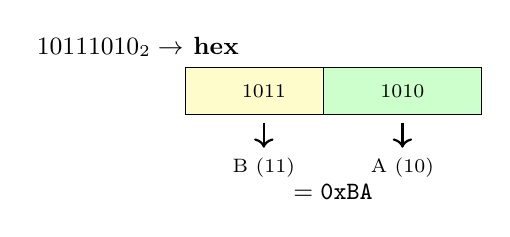
\begin{tikzpicture}[scale=0.8]
\node at (-2,1.5) [font=\small\bfseries] {$10111010_2 \rightarrow$ hex};
\node[rectangle,draw,fill=yellow!20,minimum width=2cm,minimum height=0.6cm] at (0,0.8) {\scriptsize 1011};
\node[rectangle,draw,fill=green!20,minimum width=2cm,minimum height=0.6cm] at (2.2,0.8) {\scriptsize 1010};
\draw[->,thick] (0,0.3) -- (0,-0.1) node[below,font=\scriptsize] {B (11)};
\draw[->,thick] (2.2,0.3) -- (2.2,-0.1) node[below,font=\scriptsize] {A (10)};
\node at (1.1,-0.8) [font=\small] {$= \texttt{0xBA}$};
\end{tikzpicture}
\end{center}

\begin{lstlisting}[caption={Notations en C}]
unsigned int x = 0x3A;      // 3A hex = 0011 1010 bin = 58 dec
unsigned int y = 0xFF;      // FF hex = 1111 1111 bin = 255 dec
printf("%02X\n", x);        // Affiche "3A" (toujours 2 caractères par octet)
\end{lstlisting}

\section{Représentation des Entiers}

\subsection{Entiers Non Signés (Unsigned)}

\begin{definitionbox}{Unsigned sur $w$ bits}
$\boxed{B2U_w(\vec{x}) = \sum_{i=0}^{w-1} x_i \cdot 2^i}$ \quad où $x_i \in \{0,1\}$ est le bit à la position $i$.\\[0.2em]
\textbf{Plage :} $[0, 2^w-1]$. Aucun nombre négatif représentable.
\end{definitionbox}

\begin{center}
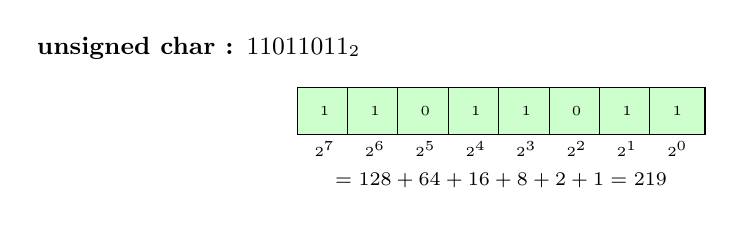
\begin{tikzpicture}[scale=0.8]
\node at (-2,1.5) [font=\small\bfseries] {unsigned char : $11011011_2$};
\foreach \i/\bit in {7/1,6/1,5/0,4/1,3/1,2/0,1/1,0/1} {
    \node[rectangle,draw,fill=green!20,minimum width=0.7cm,minimum height=0.6cm] at ({(7-\i)*0.8},0.5) {\tiny\bit};
    \node at ({(7-\i)*0.8},-0.1) [font=\tiny] {$2^{\i}$};
}
\node at (2.8,-0.6) [font=\scriptsize] {$= 128+64+16+8+2+1 = 219$};
\end{tikzpicture}
\end{center}

\begin{center}
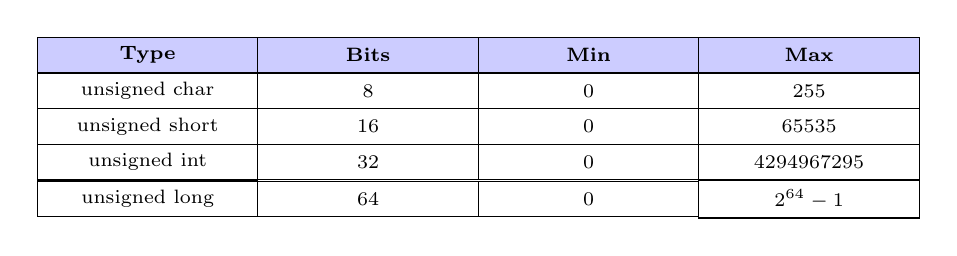
\begin{tikzpicture}[scale=0.75]
\node at (0,1.8) [font=\small\bfseries] {Plages des types unsigned};
\matrix (m) [matrix of nodes,
    nodes={rectangle,draw,minimum width=2.8cm,minimum height=0.45cm,anchor=center,font=\scriptsize},
    column sep=-\pgflinewidth, row sep=-\pgflinewidth,
    row 1/.style={nodes={fill=blue!20,font=\scriptsize\bfseries}}] at (0,0.5)
{
Type & Bits & Min & Max \\
unsigned char & 8 & 0 & 255 \\
unsigned short & 16 & 0 & 65535 \\
unsigned int & 32 & 0 & 4294967295 \\
unsigned long & 64 & 0 & $2^{64}-1$ \\
};
\end{tikzpicture}
\end{center}

\subsection{Complément à Deux (Two's Complement)}

\begin{definitionbox}{Two's complement sur $w$ bits}
$\boxed{B2T_w(\vec{x}) = -x_{w-1} \cdot 2^{w-1} + \sum_{i=0}^{w-2} x_i \cdot 2^i}$\\[0.2em]
Le bit de poids fort (MSB) $x_{w-1}$ est le \textbf{bit de signe} : 0 = positif, 1 = négatif.\\[0.2em]
\textbf{Plage :} $[-2^{w-1}, 2^{w-1}-1]$. \textbf{Asymétrie :} $|T_{min}| = |T_{max}| + 1$.
\end{definitionbox}

\begin{center}
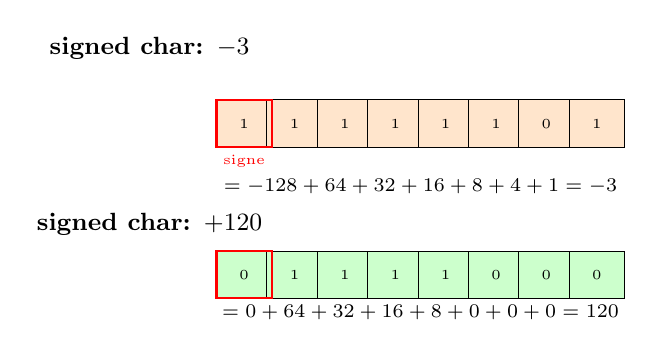
\begin{tikzpicture}[scale=0.8]
\node at (-1.5,2) [font=\small\bfseries] {signed char: $-3$};
\foreach \i/\bit in {7/1,6/1,5/1,4/1,3/1,2/1,1/0,0/1} {
    \node[rectangle,draw,fill=orange!20,minimum width=0.7cm,minimum height=0.6cm] at ({(7-\i)*0.8},0.8) {\tiny\bit};
}
\node[rectangle,draw=red,thick,minimum width=0.7cm,minimum height=0.6cm] at (0,0.8) {};
\node at (0,0.2) [font=\tiny,red] {signe};
\node at (2.8,-0.2) [font=\scriptsize] {$= -128+64+32+16+8+4+1 = -3$};
\node at (-1.5,-0.8) [font=\small\bfseries] {signed char: $+120$};
\foreach \i/\bit in {7/0,6/1,5/1,4/1,3/1,2/0,1/0,0/0} {
    \node[rectangle,draw,fill=green!20,minimum width=0.7cm,minimum height=0.6cm] at ({(7-\i)*0.8},-1.6) {\tiny\bit};
}
\node[rectangle,draw=red,thick,minimum width=0.7cm,minimum height=0.6cm] at (0,-1.6) {};
\node at (2.8,-2.2) [font=\scriptsize] {$= 0+64+32+16+8+0+0+0 = 120$};
\end{tikzpicture}
\end{center}

\begin{techbox}{Valeurs remarquables (8 bits)}
\textbf{$-1$ :} Tous les bits à 1 $\rightarrow$ \texttt{0xFF} $= 11111111_2$\\
\textbf{$T_{min} = -128$ :} Bit de signe à 1, reste à 0 $\rightarrow$ \texttt{0x80} $= 10000000_2$\\
\textbf{$T_{max} = 127$ :} Bit de signe à 0, reste à 1 $\rightarrow$ \texttt{0x7F} $= 01111111_2$\\
\textbf{Négation :} $-x = \sim x + 1$ (inverser tous les bits, ajouter 1)
\end{techbox}

\begin{center}
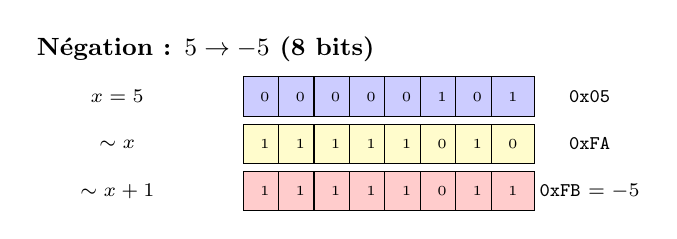
\begin{tikzpicture}[scale=0.75]
\node at (-1,2.8) [font=\small\bfseries] {Négation : $5 \rightarrow -5$ (8 bits)};
\node at (-2.5,2) [font=\scriptsize] {$x = 5$};
\foreach \i/\bit in {7/0,6/0,5/0,4/0,3/0,2/1,1/0,0/1} {
    \node[rectangle,draw,fill=blue!20,minimum width=0.55cm,minimum height=0.5cm] at ({(7-\i)*0.6},2) {\tiny\bit};
}
\node at (5.5,2) [font=\scriptsize] {\texttt{0x05}};
\node at (-2.5,1.2) [font=\scriptsize] {$\sim x$};
\foreach \i/\bit in {7/1,6/1,5/1,4/1,3/1,2/0,1/1,0/0} {
    \node[rectangle,draw,fill=yellow!20,minimum width=0.55cm,minimum height=0.5cm] at ({(7-\i)*0.6},1.2) {\tiny\bit};
}
\node at (5.5,1.2) [font=\scriptsize] {\texttt{0xFA}};
\node at (-2.5,0.4) [font=\scriptsize] {$\sim x + 1$};
\foreach \i/\bit in {7/1,6/1,5/1,4/1,3/1,2/0,1/1,0/1} {
    \node[rectangle,draw,fill=red!20,minimum width=0.55cm,minimum height=0.5cm] at ({(7-\i)*0.6},0.4) {\tiny\bit};
}
\node at (5.5,0.4) [font=\scriptsize] {\texttt{0xFB} $= -5$};
\end{tikzpicture}
\end{center}

\section{Conversions Signed $\leftrightarrow$ Unsigned}

\begin{definitionbox}{Principe de conversion}
La conversion entre signed et unsigned \textbf{préserve le motif binaire} mais change son interprétation. Aucun bit n'est modifié.
\end{definitionbox}

\begin{center}
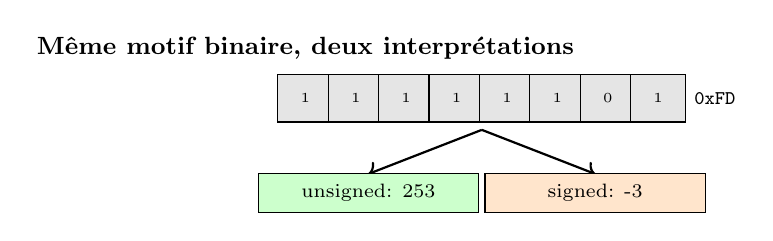
\begin{tikzpicture}[scale=0.8]
\node at (0,2.3) [font=\small\bfseries] {Même motif binaire, deux interprétations};
\foreach \i/\bit in {7/1,6/1,5/1,4/1,3/1,2/1,1/0,0/1} {
    \node[rectangle,draw,fill=gray!20,minimum width=0.7cm,minimum height=0.6cm] at ({(7-\i)*0.8},1.5) {\tiny\bit};
}
\node at (6.5,1.5) [font=\scriptsize] {\texttt{0xFD}};
\draw[->,thick] (2.8,1) -- (1,0.3);
\draw[->,thick] (2.8,1) -- (4.6,0.3);
\node[rectangle,draw,fill=green!20,minimum width=2.8cm,minimum height=0.5cm] at (1,0) {\scriptsize unsigned: 253};
\node[rectangle,draw,fill=orange!20,minimum width=2.8cm,minimum height=0.5cm] at (4.6,0) {\scriptsize signed: -3};
\end{tikzpicture}
\end{center}

\begin{techbox}{Formules de conversion (sur $w$ bits)}
\textbf{Signed $\rightarrow$ Unsigned :} $T2U_w(x) = \begin{cases} x & \text{si } x \geq 0 \\ x + 2^w & \text{si } x < 0 \end{cases}$\\[0.3em]
\textbf{Unsigned $\rightarrow$ Signed :} $U2T_w(u) = \begin{cases} u & \text{si } u \leq T_{max} \\ u - 2^w & \text{si } u > T_{max} \end{cases}$
\end{techbox}

\begin{lstlisting}[caption={Conversions en C}]
signed char sc = -1;              // 0xFF en mémoire
unsigned char uc = (unsigned char)sc;  // Toujours 0xFF, interprété comme 255
int x = -1;
unsigned int y = 0;
if (x < y)   // FAUX! x converti en unsigned: 0xFFFFFFFF > 0
    printf("x < y\n");  // N'est PAS exécuté!
\end{lstlisting}

\begin{warningbox}{Comparaisons signed/unsigned}
Quand un opérande est signed et l'autre unsigned, le signed est \textbf{implicitement converti en unsigned}. Cela peut inverser le résultat attendu des comparaisons.
\end{warningbox}

\begin{center}
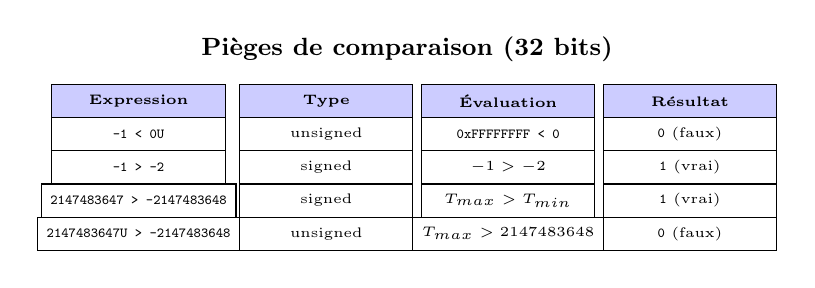
\begin{tikzpicture}[scale=0.75]
\node at (0,2.8) [font=\small\bfseries] {Pièges de comparaison (32 bits)};
\matrix (m) [matrix of nodes,
    nodes={rectangle,draw,minimum width=2.2cm,minimum height=0.42cm,anchor=center,font=\tiny},
    column sep=-\pgflinewidth, row sep=-\pgflinewidth,
    row 1/.style={nodes={fill=blue!20,font=\tiny\bfseries}}] at (0,0.8)
{
Expression & Type & Évaluation & Résultat \\
\texttt{-1 < 0U} & unsigned & \texttt{0xFFFFFFFF < 0} & \texttt{0} (faux) \\
\texttt{-1 > -2} & signed & $-1 > -2$ & \texttt{1} (vrai) \\
\texttt{2147483647 > -2147483648} & signed & $T_{max} > T_{min}$ & \texttt{1} (vrai) \\
\texttt{2147483647U > -2147483648} & unsigned & $T_{max} > 2147483648$ & \texttt{0} (faux) \\
};
\end{tikzpicture}
\end{center}

\section{Extension de Signe}

\begin{definitionbox}{Extension lors de la promotion de type}
Quand on convertit un entier de $w$ bits vers $w'$ bits ($w' > w$) :\\
\textbf{Unsigned :} Extension par zéros (zero extension) \quad \textbf{Signed :} Extension du bit de signe (sign extension)
\end{definitionbox}

\begin{center}
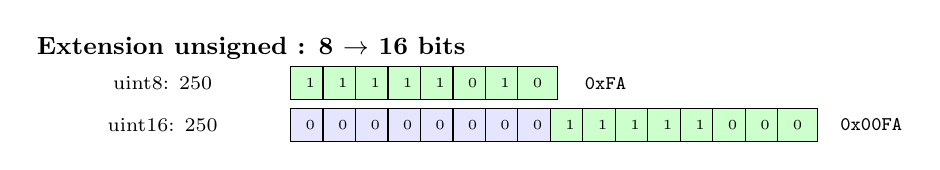
\begin{tikzpicture}[scale=0.75]
\node at (-1,2.8) [font=\small\bfseries] {Extension unsigned : 8 $\rightarrow$ 16 bits};
\node at (-2.5,2.2) [font=\scriptsize] {uint8: 250};
\foreach \i/\bit in {7/1,6/1,5/1,4/1,3/1,2/0,1/1,0/0} {
    \node[rectangle,draw,fill=green!20,minimum width=0.5cm,minimum height=0.42cm] at ({(7-\i)*0.55},2.2) {\tiny\bit};
}
\node at (5,2.2) [font=\scriptsize] {\texttt{0xFA}};
\node at (-2.5,1.5) [font=\scriptsize] {uint16: 250};
\foreach \i/\bit in {15/0,14/0,13/0,12/0,11/0,10/0,9/0,8/0} {
    \node[rectangle,draw,fill=blue!10,minimum width=0.5cm,minimum height=0.42cm] at ({(15-\i)*0.55},1.5) {\tiny\bit};
}
\foreach \i/\bit in {7/1,6/1,5/1,4/1,3/1,2/0,1/0,0/0} {
    \node[rectangle,draw,fill=green!20,minimum width=0.5cm,minimum height=0.42cm] at ({(15-\i)*0.55},1.5) {\tiny\bit};
}
\node at (9.5,1.5) [font=\scriptsize] {\texttt{0x00FA}};
\end{tikzpicture}
\end{center}

\begin{center}
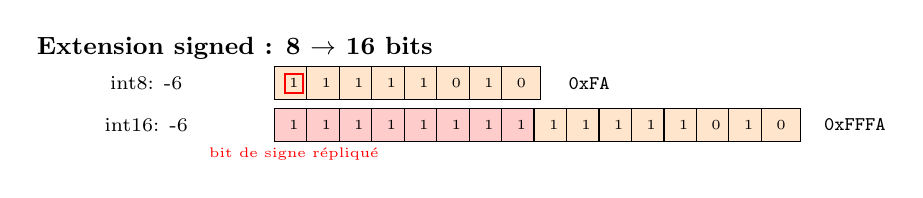
\begin{tikzpicture}[scale=0.75]
\node at (-1,2.8) [font=\small\bfseries] {Extension signed : 8 $\rightarrow$ 16 bits};
\node at (-2.5,2.2) [font=\scriptsize] {int8: -6};
\foreach \i/\bit in {7/1,6/1,5/1,4/1,3/1,2/0,1/1,0/0} {
    \node[rectangle,draw,fill=orange!20,minimum width=0.5cm,minimum height=0.42cm] at ({(7-\i)*0.55},2.2) {\tiny\bit};
}
\node[rectangle,draw=red,thick] at (0,2.2) {};
\node at (5,2.2) [font=\scriptsize] {\texttt{0xFA}};
\node at (-2.5,1.5) [font=\scriptsize] {int16: -6};
\foreach \i/\bit in {15/1,14/1,13/1,12/1,11/1,10/1,9/1,8/1} {
    \node[rectangle,draw,fill=red!20,minimum width=0.5cm,minimum height=0.42cm] at ({(15-\i)*0.55},1.5) {\tiny\bit};
}
\foreach \i/\bit in {7/1,6/1,5/1,4/1,3/1,2/0,1/1,0/0} {
    \node[rectangle,draw,fill=orange!20,minimum width=0.5cm,minimum height=0.42cm] at ({(15-\i)*0.55},1.5) {\tiny\bit};
}
\node at (9.5,1.5) [font=\scriptsize] {\texttt{0xFFFA}};
\node at (0,1) [font=\tiny,red] {bit de signe répliqué};
\end{tikzpicture}
\end{center}

\begin{lstlisting}[caption={Extension de signe en C}]
int8_t x = -6;           // 0xFA
int16_t y = x;           // 0xFFFA (bit de signe étendu)
uint8_t a = 250;         // 0xFA
uint16_t b = a;          // 0x00FA (zéros ajoutés)
int8_t neg = -1;         // 0xFF
uint32_t big = (uint8_t)neg;  // 0x000000FF (255), pas 0xFFFFFFFF
\end{lstlisting}

\section{Dépassements et Débordements}

\subsection{Overflow Unsigned}

\begin{definitionbox}{Comportement unsigned (défini par la norme C)}
L'arithmétique unsigned est définie \textbf{modulo $2^w$}. Le débordement "wrap around" est \textbf{garanti}.
$\boxed{\text{Résultat} = (\text{valeur mathématique}) \mod 2^w}$
\end{definitionbox}

\begin{center}
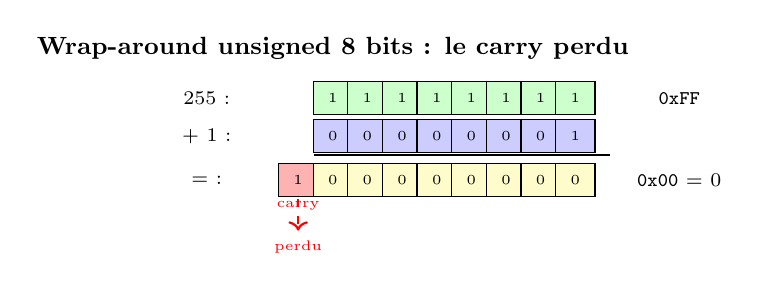
\begin{tikzpicture}[scale=0.8]
\node at (0,3) [font=\small\bfseries] {Wrap-around unsigned 8 bits : le carry perdu};
\node at (-2,2.2) [font=\scriptsize] {255 :};
\foreach \i/\bit in {7/1,6/1,5/1,4/1,3/1,2/1,1/1,0/1} {
    \node[rectangle,draw,fill=green!20,minimum width=0.5cm,minimum height=0.42cm] at ({(7-\i)*0.55},2.2) {\tiny\bit};
}
\node at (5.5,2.2) [font=\scriptsize] {\texttt{0xFF}};
\node at (-2,1.6) [font=\scriptsize] {+ 1 :};
\foreach \i/\bit in {7/0,6/0,5/0,4/0,3/0,2/0,1/0,0/1} {
    \node[rectangle,draw,fill=blue!20,minimum width=0.5cm,minimum height=0.42cm] at ({(7-\i)*0.55},1.6) {\tiny\bit};
}
\draw[thick] (-0.3,1.3) -- (4.4,1.3);
\node at (-2,0.9) [font=\scriptsize] {= :};
\node[rectangle,draw,fill=red!30,minimum width=0.5cm,minimum height=0.42cm] at (-0.55,0.9) {\tiny 1};
\node at (-0.55,0.5) [font=\tiny,red] {carry};
\foreach \i/\bit in {7/0,6/0,5/0,4/0,3/0,2/0,1/0,0/0} {
    \node[rectangle,draw,fill=yellow!20,minimum width=0.5cm,minimum height=0.42cm] at ({(7-\i)*0.55},0.9) {\tiny\bit};
}
\node at (5.5,0.9) [font=\scriptsize] {\texttt{0x00} = 0};
\draw[->,red,thick,dashed] (-0.55,0.6) -- (-0.55,0.1) node[below,font=\tiny,red] {perdu};
\end{tikzpicture}
\end{center}

\begin{lstlisting}[caption={Overflow unsigned}]
unsigned char x = 255;
x++;                      // x = 0 (défini, wrap-around: 256 mod 256 = 0)
unsigned char y = 0;
y--;                      // y = 255 (défini: -1 + 256 = 255)
// Détection d'overflow AVANT addition (sûr)
if (b > UINT_MAX - a)     // Vérifie si a + b dépasserait UINT_MAX
    printf("Overflow would occur!\n");
\end{lstlisting}

\subsection{Overflow Signed}

\begin{warningbox}{Comportement signed (Undefined Behavior)}
Le débordement d'entiers signés est un \textbf{Undefined Behavior} (UB) en C. Le compilateur peut supposer qu'il ne se produit jamais et optimiser le code en conséquence. Le résultat est \textbf{imprévisible}.
\end{warningbox}

\begin{center}
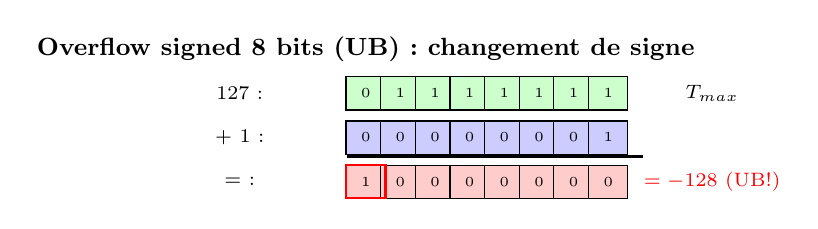
\begin{tikzpicture}[scale=0.8]
\node at (0,3.2) [font=\small\bfseries] {Overflow signed 8 bits (UB) : changement de signe};
\node at (-2,2.5) [font=\scriptsize] {127 :};
\foreach \i/\bit in {7/0,6/1,5/1,4/1,3/1,2/1,1/1,0/1} {
    \node[rectangle,draw,fill=green!20,minimum width=0.5cm,minimum height=0.42cm] at ({(7-\i)*0.55},2.5) {\tiny\bit};
}
\node at (5.5,2.5) [font=\scriptsize] {$T_{max}$};
\node at (-2,1.8) [font=\scriptsize] {+ 1 :};
\foreach \i/\bit in {7/0,6/0,5/0,4/0,3/0,2/0,1/0,0/1} {
    \node[rectangle,draw,fill=blue!20,minimum width=0.5cm,minimum height=0.42cm] at ({(7-\i)*0.55},1.8) {\tiny\bit};
}
\draw[thick] (-0.3,1.5) -- (4.4,1.5);
\node at (-2,1.1) [font=\scriptsize] {= :};
\foreach \i/\bit in {7/1,6/0,5/0,4/0,3/0,2/0,1/0,0/0} {
    \node[rectangle,draw,fill=red!20,minimum width=0.5cm,minimum height=0.42cm] at ({(7-\i)*0.55},1.1) {\tiny\bit};
}
\node[rectangle,draw=red,thick,minimum width=0.5cm,minimum height=0.42cm] at (0,1.1) {};
\node at (5.5,1.1) [font=\scriptsize,red] {$= -128$ (UB!)};
\end{tikzpicture}
\end{center}

\begin{lstlisting}[caption={Détection sûre d'overflow signed AVANT l'opération}]
#include <limits.h>
int a = 2000000000, b = 1000000000;
if ((b > 0 && a > INT_MAX - b) || (b < 0 && a < INT_MIN - b)) {
    printf("Overflow se produirait!\n");
} else {
    int sum = a + b;  // Safe
}
\end{lstlisting}

\begin{warningbox}{Bugs de sécurité réels (CVE)}
\textbf{CVE-2009-1385 (Linux kernel e1000 driver):} Un overflow d'entier permettait un buffer overflow.\\
\textbf{CVE-2021-43267 (Linux kernel TIPC):} Un overflow dans la validation de taille permettait une exécution de code.
\end{warningbox}

\section{Représentation IEEE 754 (Flottants)}

\subsection{Pourquoi les flottants ?}

Les entiers ne suffisent pas pour : très grands nombres ($1.5 \times 10^{11}$ m), très petits nombres ($9.11 \times 10^{-31}$ kg), nombres fractionnaires ($\pi$, 19.99 €).

\begin{examplebox}{Le problème de la virgule fixe}
Virgule fixe gaspille des bits : pour $0.000001$ la partie entière est inutile, pour $10^{15}$ la partie fractionnaire est inutile. \textbf{Solution :} Faire "flotter" la virgule → virgule \textbf{flottante}.
\end{examplebox}

\subsection{Nombres binaires fractionnaires}

\begin{definitionbox}{Représentation binaire fractionnaire}
$\boxed{b_m b_{m-1} \ldots b_1 b_0 \textcolor{red}{.} b_{-1} b_{-2} \ldots b_{-n} = \sum_{i=-n}^{m} b_i \times 2^i}$\\[0.2em]
Bits à gauche du point : poids $2^0, 2^1, 2^2, ...$\\
Bits à droite du point : poids $2^{-1} = 0.5$, $2^{-2} = 0.25$, $2^{-3} = 0.125$, ...
\end{definitionbox}

\begin{center}

\includegraphics[width=0.85\textwidth]{fig_01_binary_weights.pdf}
\end{center}

\begin{examplebox}{Exemple : $101.11_2 = ?$}
$101.11_2 = 1 \times 2^2 + 0 \times 2^1 + 1 \times 2^0 + 1 \times 2^{-1} + 1 \times 2^{-2} = 4 + 0 + 1 + 0.5 + 0.25 = \mathbf{5.75}$
\end{examplebox}

\subsection{Formule IEEE 754}

\begin{definitionbox}{Formule IEEE 754}
$\boxed{V = (-1)^s \times M \times 2^E}$\\[0.2em]
$s$ = Signe (0 = positif, 1 = négatif), $M$ = Mantisse (chiffres significatifs), $E$ = Exposant (puissance de 2)
\end{definitionbox}

\subsection{Structure d'un float (32 bits)}

\begin{center}
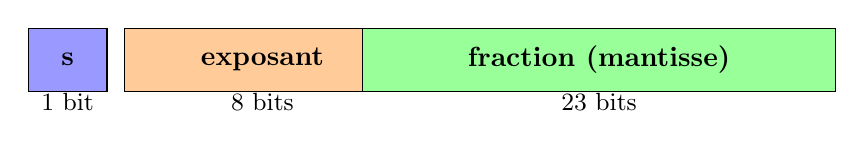
\begin{tikzpicture}[scale=0.9]
\node[rectangle,draw,fill=blue!40,minimum width=1cm,minimum height=0.8cm] at (0,0) {\textbf{s}};
\node[rectangle,draw,fill=orange!40,minimum width=3.5cm,minimum height=0.8cm] at (2.75,0) {\textbf{exposant}};
\node[rectangle,draw,fill=green!40,minimum width=6cm,minimum height=0.8cm] at (7.5,0) {\textbf{fraction (mantisse)}};
\node at (0,-0.6) [font=\small] {1 bit};
\node at (2.75,-0.6) [font=\small] {8 bits};
\node at (7.5,-0.6) [font=\small] {23 bits};
\end{tikzpicture}
\end{center}

\begin{techbox}{Décodage des champs}
\textbf{Signe :} $s = 0$ → positif, $s = 1$ → négatif\\
\textbf{Exposant biaisé :} $\text{exposant stocké} = E + 127$ donc $E = \text{exposant stocké} - 127$\\
\textbf{Mantisse avec "1 implicite" :} $M = 1.\text{fraction}$ (le "1." n'est pas stocké)
\end{techbox}

\subsection{Exemple : convertir 13.0 en float}

\begin{enumerate}
    \item \textbf{Signe :} $13.0$ positif → $s = 0$
    \item \textbf{Binaire :} $13 = 1101_2$ donc $13.0 = 1101.0_2$
    \item \textbf{Normaliser :} $1101.0_2 = 1.101_2 \times 2^3$ → $E = 3$
    \item \textbf{Exposant biaisé :} $3 + 127 = 130 = 10000010_2$
    \item \textbf{Fraction :} $101$ + 20 zéros
\end{enumerate}

\begin{center}
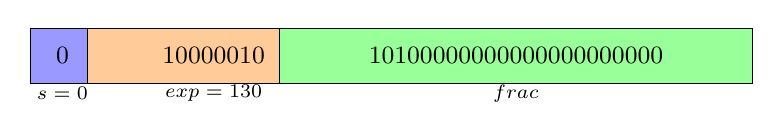
\begin{tikzpicture}[scale=0.8]
\node[rectangle,draw,fill=blue!40,minimum width=0.8cm,minimum height=0.7cm] at (0,0) {\small 0};
\node[rectangle,draw,fill=orange!40,minimum width=3.2cm,minimum height=0.7cm] at (2.4,0) {\small 10000010};
\node[rectangle,draw,fill=green!40,minimum width=6cm,minimum height=0.7cm] at (7.2,0) {\small 10100000000000000000000};
\node at (0,-0.6) [font=\scriptsize] {$s=0$};
\node at (2.4,-0.6) [font=\scriptsize] {$exp=130$};
\node at (7.2,-0.6) [font=\scriptsize] {$frac$};
\end{tikzpicture}
\end{center}

\textbf{Résultat :} \texttt{0x41500000}. \textbf{Vérification :} $(-1)^0 \times 1.101_2 \times 2^3 = 1.625 \times 8 = 13.0$ \checkmark

\subsection{Exemple : $-13.625$}

\begin{center}

\includegraphics[width=0.95\textwidth]{fig_02_ieee754_anatomy.pdf}
\end{center}

\begin{examplebox}{Décorticage de $-13.625$}
\textbf{1.} Signe : négatif → $s = 1$\\
\textbf{2.} Binaire : $13 = 1101_2$, $0.625 = 0.101_2$ → $13.625 = 1101.101_2$\\
\textbf{3.} Normalisation : $1.101101_2 \times 2^3$\\
\textbf{4.} Exposant : $3 + 127 = 130 = 10000010_2$\\
\textbf{5.} Fraction : $101101$ + 17 zéros\\
\textbf{Résultat :} \texttt{0xC15A0000}
\end{examplebox}

\subsection{Valeurs spéciales}

\begin{center}
\begin{tabular}{|c|c|l|}
\hline
\textbf{Valeur} & \textbf{Quand ?} & \textbf{Exemple en C} \\
\hline
$+0$ et $-0$ & Deux représentations de zéro & \texttt{0.0f}, \texttt{-0.0f} \\
$+\infty$ et $-\infty$ & Dépassement de capacité & \texttt{1.0f / 0.0f} \\
\textbf{NaN} & Opération indéfinie & \texttt{0.0f / 0.0f}, \texttt{sqrt(-1)} \\
\hline
\end{tabular}
\end{center}

\begin{warningbox}{NaN : Not a Number}
NaN n'est égal à rien, même pas à lui-même ! Utiliser \texttt{isnan(x)} pour tester.
\begin{lstlisting}[numbers=none]
float x = 0.0f / 0.0f;   // x est NaN
if (x == x)              // FAUX! NaN != NaN
if (isnan(x))            // Correct
\end{lstlisting}
\end{warningbox}

\subsection{Les pièges des flottants}

\begin{warningbox}{Piège n°1 : Représentation inexacte}
$0.1_{10} = 0.0001100110011..._2$ (infini !). Le motif "0011" se répète → erreur d'arrondi.
\end{warningbox}

\begin{warningbox}{Piège n°2 : Ne JAMAIS comparer avec ==}
\begin{lstlisting}[numbers=none]
float a = 0.1f + 0.2f, b = 0.3f;
if (a == b) ...               // DANGER! Peut être faux
if (fabsf(a - b) < 0.00001f)  // Correct: comparer avec tolérance
\end{lstlisting}
\end{warningbox}

\begin{warningbox}{Piège n°3 : Addition non associative}
\begin{lstlisting}[numbers=none]
float a = (3.14f + 1e10f) - 1e10f;   // = 0.0 !
float b = 3.14f + (1e10f - 1e10f);   // = 3.14
\end{lstlisting}
\end{warningbox}

\subsection{Cas réel : Patriot Missile (1991)}

\begin{center}

\includegraphics[width=0.95\textwidth]{fig_04_patriot_missile.pdf}
\end{center}

\begin{infobox}{Ce qui s'est passé}
\textbf{Date :} 25 février 1991, Guerre du Golfe, Dhahran, Arabie Saoudite.\\
\textbf{Bug :} L'horloge comptait en incréments de $0.1$ s approximé sur 24 bits.\\
\textbf{Après 100 heures :} Erreur cumulée $\approx 0.34$ s. À $1676$ m/s → erreur de $\approx 570$ m.\\
\textbf{Conséquence :} Le Scud n'a pas été intercepté. \textbf{28 soldats tués.}
\end{infobox}

\subsection{Application en Intelligence Artificielle}

\begin{center}

\includegraphics[width=0.95\textwidth]{fig_05_softmax_underflow.pdf}
\end{center}

\begin{infobox}{Le problème du softmax}
$\text{softmax}(x)_i = \frac{e^{x_i}}{\sum_{j} e^{x_j}}$ est utilisé partout en IA.\\
\textbf{Problème :} $e^{1000} = +\infty$ (overflow), $e^{-1000} = 0$ (underflow) → NaN\\
\textbf{Solution :} Soustraire le maximum avant de calculer (numériquement stable).
\end{infobox}

\begin{techbox}{Formats modernes pour l'IA}
\begin{center}
\begin{tabular}{|l|c|l|}
\hline
\textbf{Format} & \textbf{Bits} & \textbf{Usage} \\
\hline
float32 & 32 & Standard, haute précision \\
float16 & 16 & Entraînement GPU accéléré \\
bfloat16 & 16 & Google TPU \\
int8 & 8 & Inférence quantifiée \\
\hline
\end{tabular}
\end{center}
\end{techbox}


\section{Bonnes Pratiques}

\subsection{Types portables}

\begin{techbox}{Utiliser les types de taille fixe (\texttt{<stdint.h>})}
\begin{center}
\begin{tabular}{|l|l|l|}
\hline
\textbf{Type signé} & \textbf{Type non signé} & \textbf{Taille} \\
\hline
\texttt{int8\_t} & \texttt{uint8\_t} & 8 bits \\
\texttt{int16\_t} & \texttt{uint16\_t} & 16 bits \\
\texttt{int32\_t} & \texttt{uint32\_t} & 32 bits \\
\texttt{int64\_t} & \texttt{uint64\_t} & 64 bits \\
\hline
\end{tabular}
\end{center}
\end{techbox}

\begin{lstlisting}[caption={Types portables}]
#include <stdint.h>
#include <inttypes.h>
uint32_t counter = 0;
printf("counter = %" PRIu32 "\n", counter);
\end{lstlisting}

\subsection{Éviter les pièges signed/unsigned}

\begin{lstlisting}[caption={Comparaisons sûres}]
int index = -1;
unsigned int limit = 100;
if (index >= 0 && (unsigned int)index < limit)  // BON: cast explicite
    printf("Index valide\n");
\end{lstlisting}

\subsection{Options de compilation recommandées}

\begin{lstlisting}[caption={Options gcc},language=bash]
gcc -Wall -Wextra -Werror -Wsign-compare -fsanitize=undefined -g prog.c
\end{lstlisting}

\end{document}
